\chapter{Implementierung}
\label{chapter:Dokumentation-Implementierung}

\section{Hardwareerweiterung}
\label{section:Dokumentation-Implementierung-Hardwareerweiterung}

\subsection{Register}
\label{subsection:Dokumentation-Implementierung-Hardwareerweiterung-Register}

\begin{description}
    \item[BUFFER\_ONE] immer voller Buffer, bitgenau
    \item[BUFFER\_TWO] füllt \texttt{BUFFER\_ONE}, wird mit Speicherzellen gefüllt
    \item[FILLED] Füllstand von \texttt{BUFFER\_TWO}
    \item[FILLEDTMP] Zwischenspeicher
    \item[TABELLENANFANG] Startadresse der Ergebnistabelle
    \item[KANALNR] Nummer des aktuellen Kanals
\end{description}

\subsection{ALU"=Operationen}
\label{subsection:Dokumentation-Implementierung-Hardwareerweiterung-AluOps}

\begin{description}
    \item[MUL] $ALUresult \gets A \cdot B$
    \item[SR.B] $ALUresult \gets 0@B_{31..1}$
    \item[AND] $ALUresult \gets A \&\& B$
\end{description}

Die hinzugefügten Operationen waren bereits im Simulator implementiert, sodass wir sie lediglich "`aktivieren"' mussten.

\subsection{Konstanten}
\label{subsection:Dokumentation-Implementierung-Hardwareerweiterung-Konstanten}

\begin{itemize}
    \item $(14)_{10} = (e)_{16} = (1110)_2$
    \item $(2^{31})_{10}$
    \item $(2^{28})_{10}$
    \item $(2^{16})_{10}$
    \item $(2^5)_{10}$
    \item $(2^4)_{10}$
    \item $(2)_{10}$
\end{itemize}

\subsection{Konfigurationsdatei}
\label{subsection:Dokumentation-Implementierung-Hardwareerweiterung-Konfigurationsdatei}

Mit Hilfe der bereitgestellten Beispiele konnte eine Erweiterungsdatei für die die oben genannten Erweiterungen erstellt werden. Diese kann in den Simulator geladen werden (siehe \autoref{chapter:Dokumentation-Simulation}), wodurch die simulierte Hardware um die o.g. Komponenten (ALU"=Operationen, Konstanten, \ldots) erweitert wird.

Zwar besitzt der Simulator eine grafische Oberfläche zum Erstellen dieser Kon\-fi\-gu\-ra\-tions\-datei, jedoch war die Bedienung unschlüssig und ein direktes Verfassen der Konfigurationsdatei per Hand um ein vielfaches schneller.

Die Erweiterungskonfiguration befindet sich in \autoref{chapter:Anhang-Konfiguration}.

In \autoref{figure:Dokumentation-Implementierung-Hardwareerweiterung-Layout} befindet sich eine grafische Übersicht über die erweiterte Minimax"=Maschine. Erweiterungen zur Basismaschine wurden farblich hervorgehoben.

\begin{figure}[htb]
    \centering
    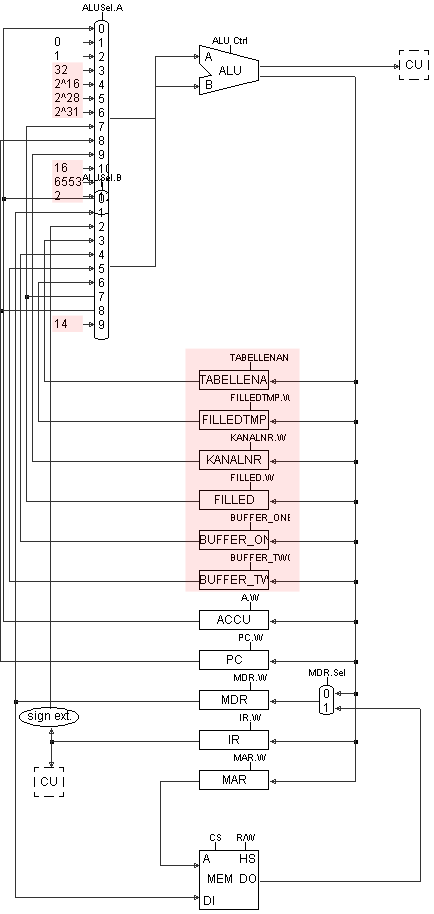
\includegraphics[width=0.65\textwidth]{dokumentation/res/minimax_maschinenlayout_highlight.png}
    \caption{Grafische Übersicht der erweiterten Minimax"=Maschine}
    \label{figure:Dokumentation-Implementierung-Hardwareerweiterung-Layout}
\end{figure}

\clearpage

\subsection{Maschinencodierung}
\label{subsection:Dokumentation-Implementierung-Hardwareerweiterung-Maschinencodierung}

\textbf{ALU"=Operationen:}

\begin{tabular}{lc}
    Operation & Code \\
    \hline
    ADD       & 000 \\
    SUB.B     & 001 \\
    TRANS.A   & 010 \\
    TRANS.B   & 011 \\
    MUL       & 100 \\
    SR.B      & 101 \\
    AND       & 110 \\
\end{tabular}

\textbf{ALUSel.A:}

\begin{tabular}{lcc}
    Quelle               & Code & Eingang \\
    \hline
    ACCU                 & 0000 &  0 \\
    0                    & 0001 &  1 \\
    1                    & 0010 &  2 \\
    (32)_{10}            & 0011 &  3 \\
    (2^{16})_{10}        & 0100 &  4 \\
    (2^{28})_{10}        & 0101 &  5 \\
    (2^{31})_{10}        & 0110 &  6 \\
    FILLED               & 0111 &  7 \\
    PC                   & 1000 &  8 \\
    KANALNR              & 1001 &  9 \\
    (2^4)_{10}           & 1010 & 10 \\
    (2)_{10}             & 1011 & 11 \\
\end{tabular}

\textbf{ALUSel.B:}

\begin{tabular}{lcc}
    Quelle        & Code & Eingang \\
    \hline
    ACCU          & 0000 &  0 \\
    MDR           & 0001 &  1 \\
    AT(signext)   & 0010 &  2 \\
    TABELLENANF   & 0011 &  3 \\
    BUFFER\_ONE   & 0100 &  4 \\
    BUFFER\_TWO   & 0101 &  5 \\
    FILLEDTMP     & 0110 &  6 \\
    FILLED        & 0111 &  7 \\
    PC            & 1000 &  8 \\
    (14)_{10}     & 1001 &  9 \\
\end{tabular}

\section{Algorithmus}
\label{section:Dokumentation-Implementierung-Algorithmus}

Die prinzipielle Funktionsweise des Algorithmus ist bereits in \autoref{subsection:Pflichtenheft-SystemtechnischeLoesung-Loesungsansatz-Ansatz2} von \autoref{part:Pflichtenheft} beschrieben worden. Hier soll noch auf einige Aspekte im Detail eingegangen werden.

\textbf{aktueller Speicherblock < Tabellenanfang:}

Dieser Teil ist in dem Label "`EndCheck"' kodiert und der Bedingung:

\begin{verbatim}
IF TABELLENANFANG - PC == 0
          0,GOTO NextCell
          1,GOTO END
\end{verbatim}

Der aktuelle Speicherblock wird dabei im PC gespeichert, da dieser sonst nur für das eine \texttt{IFETCH} am Anfang benötigt wird und somit zur freien Verfügung steht.\\
Die Bedingung wird mehrfach überprüft, da der PC an verschiedenen Stellen im Code inkrementiert wird, insbesondere bei den Sprüngen über den Header.

\textbf{nächsten Speicherblock laden}

Der Speicher wird in den \texttt{BUFFER\_TWO} geladen. Das passiert in Zeile 20 der RT"=Notation in \autoref{chapter:Anhang-RtNotation}.

\textbf{Erste 4 Bit im Zwischenspeicher == CONST\_SEQ}

Wird in der Zeile \texttt{IF STARTSEQ - ACCU == 0} überprüft. Die beiden Befehle:

\begin{verbatim}
ACCU <- 14 + 1
ACCU <- BUFFER_ONE && ACCU
\end{verbatim}

sorgen dafür, dass nur die ersten 15 Bit (die der Startsequenz entsprechen) aus \texttt{BUFFER\_ONE} im \texttt{ACCU} stehen.

\textbf{[TABELLENANFANG+KANALNR]=M[TABELLENANFANG+KANALNR]+1}

Im Datenteil wird dieser Befehl nicht mehr ausgeführt, da die Speicheroperation zu teuer ist. Stattdessen wird solange MDR inkrementiert, bis der Datenteil zu Ende ist und erst dann wird der Inhalt des MDR in die Speicherzelle mit der Adresse\linebreak \texttt{M[TABELLENANFANG+KANALNR]} geschrieben.

\textbf{einen Bit weitergehen}

ist eine Shift-Operation auf \texttt{BUFFER\_ONE}, wobei zusätzlich ein Bit aus \texttt{BUFFER\_TWO} nachgeladen wird. Das passiert in den Zeilen:

\begin{verbatim}
BUFFER_ONE <- shiftr BUFFER_ONE
ACCU <- BUFFER_TWO && 00000001
ACCU <- ACCU * 2^31
BUFFER_ONE <- BUFFER_ONE + ACCU
BUFFER_TWO <- shiftr BUFFER_TWO
\end{verbatim}

Dabei muss erst sichergestellt werden, dass im \texttt{ACCU} nur ein Bit steht, da sonst durch die Multiplikation ein Überlauf produziert wird.

\textbf{Alle Bits im aktuellen Speicherblock durchgegangen}

Die aktuelle Anzahl im \texttt{BUFFER\_TWO} wird in \texttt{FILLED} gespeichert. Die Bedingung findet sich in dieser Zeile:

\begin{verbatim}
IF FILLED == 0
          0,GOTO HeadChk
          1,GOTO EndCheck
\end{verbatim}

\textbf{Jump 32 Bit}

Im \texttt{BUFFER\_ONE} ist der aktuelle bitgenaue Speicherinhalt gespeichert. Angefangene Speicherzellen werden in \texttt{BUFFER\_TWO} gespeichert, das beim Shiften mit Nullen nachgefüllt wird. Da genau 32 Bit, also eine Registerbreite, gesprungen werden muss, wird der Inhalt von \texttt{BUFFER\_TWO} in \texttt{BUFFER\_ONE} kopiert. Die Nullen werden dabei durch eine Addition mit dem passend geshifteten Inhalt der Speicherzelle ersetzt.

\pagebreak

Folgende Grafik / Tabelle dient zur Visualisierung:

\begin{tabular}{|l|l|}
\multicolumn{2}{l}{Ist-Zustand:}\\
\hline
Speicher   & \texttt{ccccccccccccbbbbbbbbbbbbbbbbbbbb}\\
\hline
\texttt{BUFFER\_ONE} & \texttt{egalegalegalegalegalegalegalegal}\\
\hline
\texttt{BUFFER\_TWO} & \texttt{00000000000000000000aaaaaaaaaaaa}\\
\hline
\multicolumn{2}{l}{}\\
\multicolumn{2}{l}{Soll-Zustand:}\\
\hline
Speicher   & \texttt{ccccccccccccbbbbbbbbbbbbbbbbbbbb}\\
\hline
\texttt{BUFFER\_ONE} & \texttt{bbbbbbbbbbbbbbbbbbbbaaaaaaaaaaaa}\\
\hline
\texttt{BUFFER\_TWO} & \texttt{00000000000000000000cccccccccccc}\\
\hline
\end{tabular}

Dabei werden die Register \texttt{FILLEDTMP}, und \texttt{ACCU} zur Zwischenspeicherung genutzt. Wenn ein "`c-Teil"' (\texttt{FILLED = 0}) nicht vorhanden ist, wird auch nicht geshiftet. Siehe Zeilen 28-55 und 78-107 der RT"=Notation in \autoref{chapter:Anhang-RtNotation}.

\textbf{KANALNR speichern (16 Bit)}

Da die Kanalnummer nur 16 Bit lang ist, dürfen nur diese aus dem \texttt{BUFFER\_ONE} übernommen werden. Das passiert mit folgendem Code:

\begin{verbatim}
KANALNR <- BUFFER_ONE && 0000ffff
\end{verbatim}

In dem Flussdiagramm impliziert die Speicherung der Kanalnummer auch einen 16 Bit Sprung über die Kanalnummer. Das ist im Algorithmus nicht der Fall. Deswegen wird mit einer Schleife 16-mal geshiftet (auf die gleiche Art wie im Data-Teil).





\section{Steuertabelle}
\label{section:Dokumentation-Implementierung-Steuertabelle}

Da der Algorithmus bereits in der maschinennahen RT"=Notation verfasst wurde, konnte die Steuertabelle aus diesem mit Hilfe der Maschinencodierung (s.o.) direkt abgeleitet werden. Die Steuertabelle inklusive RT"=Notation befindet sich in \autoref{chapter:Anhang-Steuertabelle}.
